\documentclass[12pt]{article}

\usepackage[dvips,letterpaper,margin=0.75in,bottom=0.75in]{geometry}
\usepackage{cite}
\usepackage{slashed}
\usepackage{graphicx}
\usepackage{amsmath}

\usepackage[american,fulldiode]{circuitikz}
\usetikzlibrary{calc}

\begin{document}
\ctikzset{bipoles/thickness=1}
\ctikzset{bipoles/length=.8cm}

\title{Lab 3: Audio Amplifier}

\maketitle

\section{Pre-lab}

No pre-lab calculations.

\section{Introduction}

In this lab, you will build an audio power amplifier capable of driving a $8~\rm \Omega$ speaker the way it was meant to be driven... loudly!  You will need this device again next week, so build your circuit on a small protoboard that can be put aside for reuse next week.

We will be using the BD139 (npn) and BD140 (pnp) complementary power transistors for this lab (See Fig.~\ref{fig:bdpackage} and Fig.~\ref{fig:bdphoto}.  Each transistor is mounted on a heatsink.  During normal operation, the transistors can become very hot.  {\bf Do not touch the transistors or you might burn yourself!}  Instead, handle them by the wires and the heatsink without touching the transistor itself.

\begin{figure}[htbp]
\begin{center}
\begin{tabular}{cc}
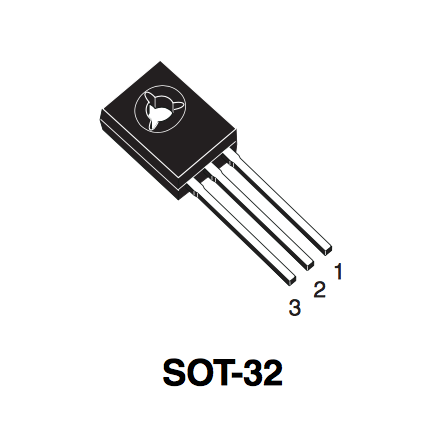
\includegraphics[width=0.30\textwidth]{figs/bd139140_package.png} &
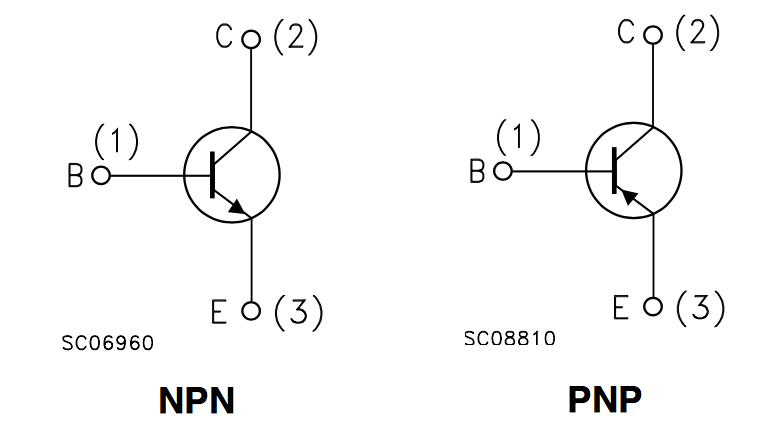
\includegraphics[width=0.50\textwidth]{figs/bd139140_pinout.png} \\
\end{tabular}
\end{center}
\caption{The SOT-32 package (left) and pinout (right) used by the BD139 (npn) and BD140 (pnp) used in this lab.  For this lab, the transistor heat sink is mounted below the device as oriented in this photo, with part number on the side facing us.}
\label{fig:bdpackage}
\end{figure}

\begin{figure}[htbp]
\begin{center}
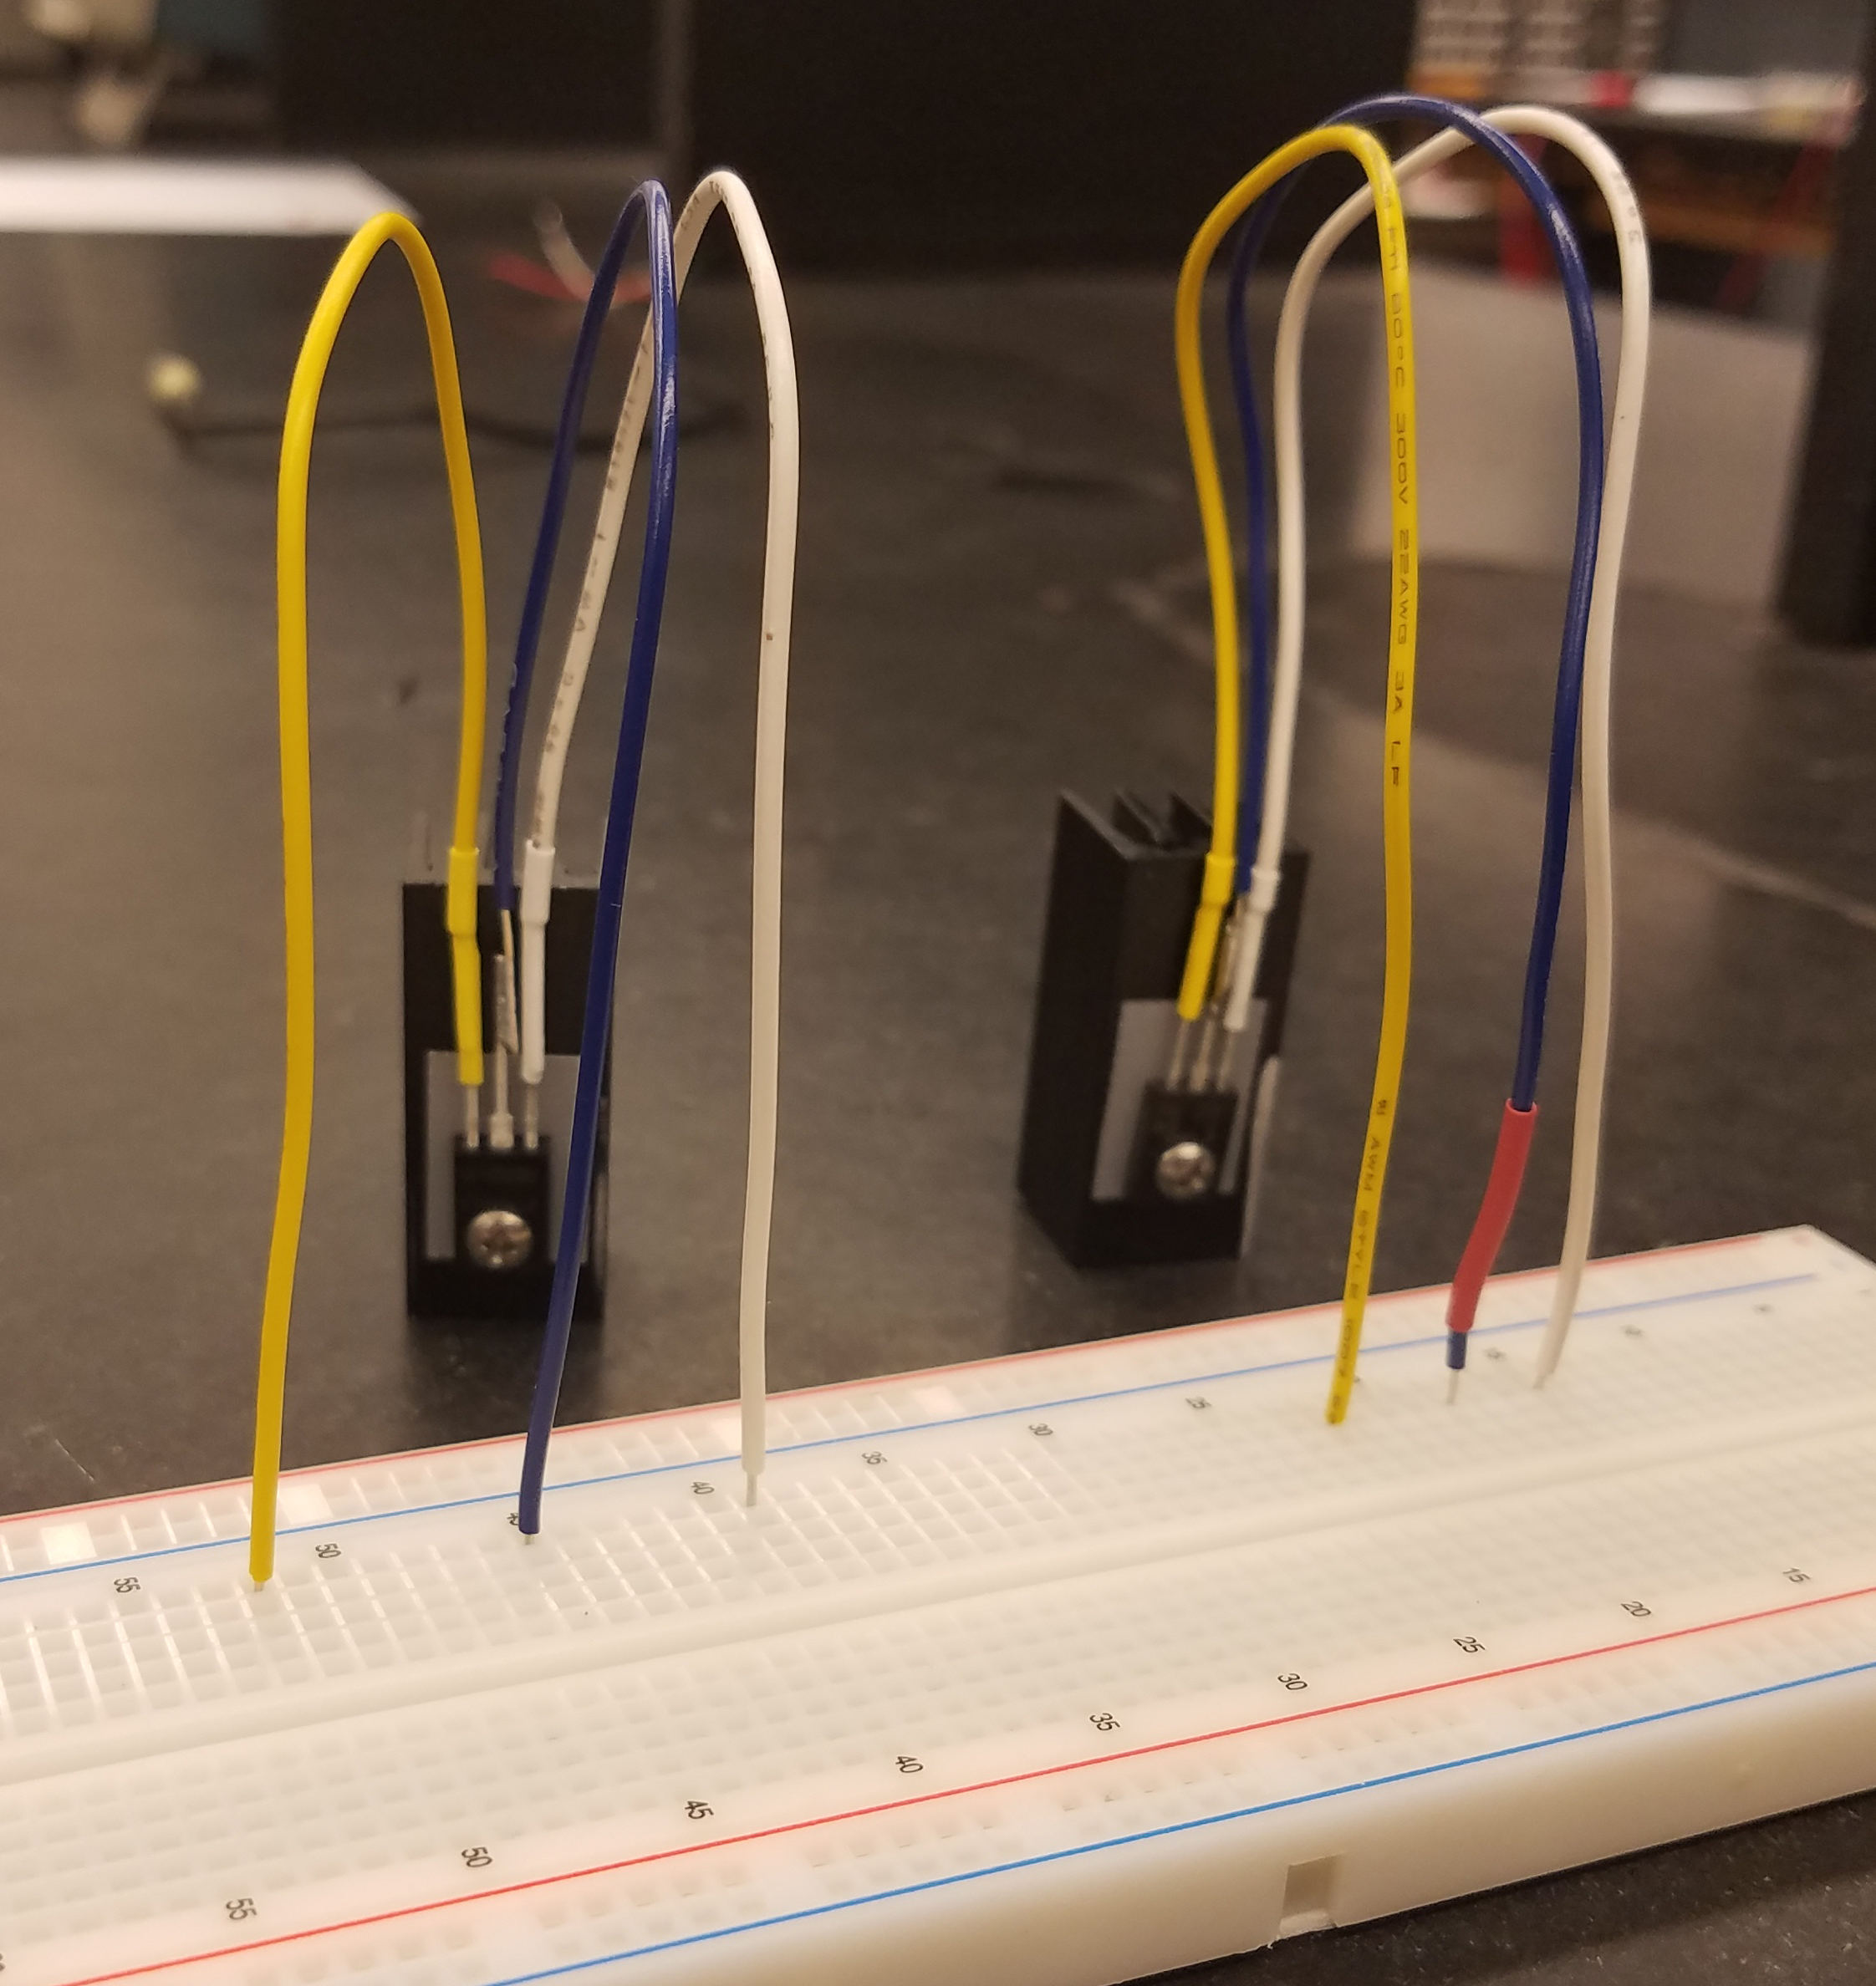
\includegraphics[height=0.35\textheight]{figs/bd139140_photo.jpg} 
\end{center}
\caption{The BD140 (left) and BD139 (right) power transistors as prepared for this lab.  Both transistors are mounted on an aluminum heat sink with an electrically insulating thermally conductive pad.  The NPN version (BD139), located at the right of the photo, is identifiable by the additional section of red heat shrink tubing on the end of the blue (collector) wire, or by using a magnifying glass to read the part number.  For both transistors, as shown in the photo, the pinout from left to right is base (yellow), collector (blue), emitter (white).}
\label{fig:bdphoto}
\end{figure}

For low-power circuits, one can (sometimes) get away with making adjustments while leaving the circuit powered.  This is not a low-power circuit.  {\bf Do not make any adjustments while the circuit is powered.}  Power down your DC supply, make your adjustments, and then power it back up.

\section{Power Amplification}

Build the emitter follower in Fig.~\ref{fig:classb} using $R_L=10~\rm k\Omega$, 
and a BD139 NPN power-transistor.  Provide $V_{\rm CC}=8~\rm V$ with your bench-top DC power supply.  Use your function generator to drive the input $v_{\rm in}$ with a $900~\rm Hz$ sinusoidal with peak-to-peak voltage of $3~\rm V$.  Observe the output with your oscilloscope. 

In this configuration, the transistor is only in the active region when the input signal is one diode drop above ground.  As a result, you only see a bit less than the top half of the sine wave.

We've already seen a solution to this problem in the transistor lab:  we AC couple the input signal and DC bias the transistor into it's active region  (See Fig.~\ref{fig:follower}).   This is called a Class A amplifier.
The Class A amplifier has a major shortcoming that becomes important when dealing with power transistors:  the DC bias current wastes a lot of power that is not needed for amplification.  In this lab, we'll explore other options for providing amplification.

\begin{figure}[htbp]
\begin{center}
\begin{circuitikz}[american,line width=1pt]
\draw (0,0) node[npn](npn){$Q_1$};
\draw (npn.C) to[short,-o] ++(0,0.5) node[right]{$V_{\rm CC}$};
\draw (npn.E) to[short] ++(0.5,0) to[short,-o] ++(0.5,0) node[right]{$v_{\rm out}$};
\draw (npn.E) to[R,l=$R_L$] ++(0,-1.5) node[ground,yscale=2.0]{};
\draw (npn.B) to[short,-o] ++(-0.5,0) node[left]{$v_{\rm in}$};
\end{circuitikz} 
\caption{An emitter-follower power amplification stage.}
\label{fig:classb}
\end{center}
\end{figure}

\begin{figure}[htbp]
\begin{center}
\begin{circuitikz}[line width=1pt]
\draw
%(2,4) node[right]{$P_2$} to[diode,l=$D$,o-o] (2,2) node[right] {$P_1$} to[resistor,l=$R$,-o](2,0) node[right]{$G$} -- (0,0)
%(2,0) -- ++(0,0) node[ground,yscale=2.0]{}
(0,0) node[npn](npn1){} 
(npn1.B) -- ++(-0.5,0) coordinate(A) to [R,l_=$R_2$,*-] ++(0,-2) coordinate(B) 
(npn1.E) to[short,*-o] ++(1.0,0) node[right]{$v_{\rm out}$}
(npn1.E) to[R,l=$R_{\rm E}$,*-*] ++(0,-1.5) node[ground,yscale=2.0]{} -| (B)
(npn1.C) to[short,-*] ++(0,1.25) coordinate(C) to[short] ++(0,.5) node[right]{$V_{\rm CC}$}
(A) to[R,l=$R_1$] ++ (0,2) -| (C)
(npn1.C) to[short,-o] ++(0,1.75) node[right]{$V_{\rm CC}$}
(A) to[C,l=$C$,-o] ++ (-2.0,0) node[left]{$v_{\rm in}$}
;
\end{circuitikz} 
\caption{The DC biased emitter follower circuit you built for the transistor lab.}
\label{fig:follower}
\end{center}
\end{figure}

\section{Push-pull Amplifier}

\begin{figure}[htbp]
\begin{center}
\begin{circuitikz}[american,line width=1pt]
\draw (0,0) node[pnp](pnp){$Q_2$};
\draw ++(0,2) node[npn](npn){$Q_1$}; 
\draw (npn.C) to[short,-o] ++(0,0.5) node[right]{$V_{\rm CC}$};
\draw (pnp.C) to[short,-o] ++(0,-0.5) node[right]{$V_{\rm EE}$};
\path (pnp.E) -- coordinate[midway](X) ( npn.E);
\draw (pnp.E) to[short,-*] (X) to[short] (npn.E);
\draw (X) to[short] ++(1.5,0) coordinate(X) to[short,-o] ++(0.5,0) node[right]{$v_{\rm out}$};
\draw (X) to[R,l=$R_L$] ++(0,-1.5) node[ground,yscale=2.0]{};
\path (pnp.B) -- coordinate[midway](X) ( npn.B);
\draw (npn.B) to[short,-*] (X) to[short] (pnp.B);
\draw (X) to[short,-o] ++(-1.5,0) node[left]{$v_{\rm in}$};
\end{circuitikz} 
\caption{A push-pull power amplification stage.}
\label{fig:pushpull}
\end{center}
\end{figure}

The circuit in Fig.~\ref{fig:pushpull} is called a push-pull amplifier.  The NPN transistor is in it's active region when the signal is one diode drop above ground, and the PNP transistor is in it's active region when the signal is one diode drop below ground.  In between, however, neither transistor is active and distortion, referred to as {\em cross-over distortion} results.  Build the circuit in Fig.~\ref{fig:pushpull} using 
a BD139 (npn) transistor and a BD140 (pnp) transistor using $R_L=10~\rm k\Omega$.  Use your DC power supply to provide $V_{\rm CC}=8~\rm V$ and $V_{\rm CC}=-8~\rm V$.  Use your function generator to drive the input $v_{\rm in}$ with a $900~\rm Hz$ sinusoidal with peak-to-peak voltage of $3~\rm V$.  Observe the output at $v_{\rm out}$ with your oscilloscope.   You should see both halves of the sine wave, but with clear distortion from the cross-over region.

\section{Push-pull Amplifier with Follower}

Using an LM741 op-amp (pinout in Fig.~\ref{fig:lm741layout}) add a follower stage to your circuit as shown in Fig.~\ref{fig:ineffective}.  Use $R_D=470~\rm \Omega$.  This follower will have no effect on the output (yet!) so confirm that it is working by observing the sine wave with cross-over distortion at the output.

At this point, you are ready to hook up your speaker in place of the resistor $R_{\rm L}$.  You should hear a tone.  You can adjust the voltage and frequency on your function generator to change the tone and volume.

\begin{figure}[htbp]
\begin{center}
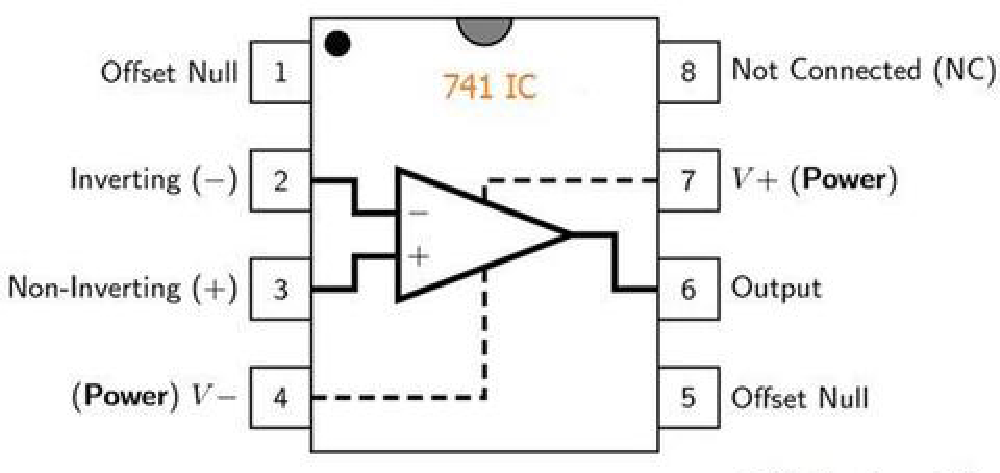
\includegraphics[height=0.15\textheight]{figs/lm741.pdf} 
\end{center}
\caption{The LM741 8-DIP layout.}
\label{fig:lm741layout}
\end{figure}

\begin{figure}[htbp]
\begin{center}
\begin{circuitikz}[american,line width=1pt]
\draw (0,0) node[pnp](pnp){$Q_2$};
\draw ++(0,2) node[npn](npn){$Q_1$}; 
\draw (-4,1) node[op amp,yscale=1](opamp){} ;
\draw (npn.C) to[short,-o] ++(0,0.5) node[right]{$V_{\rm CC}$};
\draw (pnp.C) to[short,-o] ++(0,-0.5) node[right]{$V_{\rm EE}$};
\path (pnp.E) -- coordinate[midway](X) ( npn.E);
\draw (pnp.E) to[short,-*] (X) to[short] (npn.E);
\draw (X) to[short] ++(1.5,0) coordinate(A) to[short,-o] ++(0.5,0) node[right]{$v_{\rm out}$};
\draw (A) to[R,l=$R_L$,*-] ++(0,-1.5) node[ground,yscale=2.0]{};
\path (pnp.B) -- coordinate[midway](B) ( npn.B);
\draw (npn.B) to[short,-*] (B) to[short] (pnp.B);
\draw (opamp.out) to[R,l=$R_D$] ++(1.25,0) coordinate(C) to[short] (B);
\draw (opamp.-) to[short] ++ (0,+2.5)  coordinate(X);
\draw let \p1 = (C), \p2=(X) in coordinate(Y) at (\x1,\y2);
\draw (X) to[short] (Y);
%feedback includes push-pull stage:
%\draw (Y)  -| (A);
%feedback does not include push-pull stage:
\draw (Y) to[short,-*] (C);
% input at first op mp
\draw (opamp.+) to[short,-o] ++(-.5,0) node[left]{$v_{\rm in}$};
%\draw (A) node[right]{A};
%\draw (B) node[right]{B};
%\draw (C) node[right]{C};
%\draw (D) node[right]{D};
\end{circuitikz} 
\caption{Push-pull power amplifier with (ineffective) follower.}
\label{fig:ineffective}
\end{center}
\end{figure}


\section{Feedback}

\begin{figure}[htbp]
\begin{center}
\begin{circuitikz}[american,line width=1pt]
\draw (0,0) node[pnp](pnp){$Q_2$};
\draw ++(0,2) node[npn](npn){$Q_1$}; 
\draw (-4,1) node[op amp,yscale=1](opamp){} ;
\draw (npn.C) to[short,-o] ++(0,0.5) node[right]{$V_{\rm CC}$};
\draw (pnp.C) to[short,-o] ++(0,-0.5) node[right]{$V_{\rm EE}$};
\path (pnp.E) -- coordinate[midway](X) ( npn.E);
\draw (pnp.E) to[short,-*] (X) to[short] (npn.E);
\draw (X) to[short] ++(1.5,0) coordinate(A) to[short,-o] ++(0.5,0) node[right]{$v_{\rm out}$};
\draw (A) to[R,l=$R_L$,*-] ++(0,-1.5) node[ground,yscale=2.0]{};
\path (pnp.B) -- coordinate[midway](B) ( npn.B);
\draw (npn.B) to[short,-*] (B) to[short] (pnp.B);
\draw (opamp.out) to[R,l=$R_D$] ++(1.25,0) coordinate(C) to[short] (B);
\draw (opamp.-) to[short] ++ (0,+2.5)  coordinate(X);
\draw let \p1 = (C), \p2=(X) in coordinate(Y) at (\x1,\y2);
\draw (X) to[short] (Y);
%feedback includes push-pull stage:
\draw (Y)  -| (A);
%feedback does not include push-pull stage:
%\draw (Y) to[short,*-*] (C);
% input at first op mp
\draw (opamp.+) to[short,-o] ++(-.5,0) node[left]{$v_{\rm in}$};
%\draw (A) node[right]{A};
%\draw (B) node[right]{B};
%\draw (C) node[right]{C};
%\draw (D) node[right]{D};
\end{circuitikz} 
\caption{Push-pull power amplifier featuring cross-over distortion limiting feedback.}
\label{fig:ppwfeedback}
\end{center}
\end{figure}

An effective technique for dramatically reducing feedback distortion is to use feedback.  With the circuit powered down, move the feedback from just after $R_L$ to $v_{\rm out}$ instead, as shown in Fig.~\ref{fig:ppwfeedback}.  Power your circuit and you should see (with your oscilloscope) and hear a dramatic reduction in the cross-over distortion.

\section{Feedback}

Now build the circuit in Fig.~\ref{fig:full} with $R_1=1~\rm k\Omega$, $R_2=18~\rm k\Omega$, and a variable 10k pot for $R_{\rm V}$.  As this circuit will provide voltage gain, it is now imperative that we remove high-frequency feedback, which is the role of the capacitor $C=1~\rm nF$.  I found that $R_D=470~\Omega$ gave the best overall performance.

It will help to build the circuit to the right of $R_{\rm V}$ first (omit the follower) and test that it works with the function generator to provide a voltage gain of 18.   Then connect the variable resister and test that you can vary the gain.  Then build and test the follower as a separate circuit, and finally connect the output of the follower to the rest of the circuit.

Once you build and test this circuit, and if you trust your work, you should be able to play music from your phone by attaching a phone jack between ground and $v_{\rm in}$... but ask your TA for help!
If you find you need more gain, you can increase $R_2$ to $~50~\rm k\Omega$.


Remembering to power down the circuit when reconfiguring, try playing music with the negative feedback taken after the push-pull stage (as in Fig.~\ref{fig:full}) and with the negative feedback taken before the push-pull stage (as in Fig.~\ref{fig:fullnofeedback}.  You should hear a clear difference.  That is the power of feedback!

\begin{figure}[htbp]
\begin{center}
\begin{circuitikz}[american,line width=1pt]
\draw (0,0) node[pnp](pnp){$Q_2$};
\draw ++(0,2) node[npn](npn){$Q_1$}; 
\draw (-4,1) node[op amp,yscale=1](opamp){} ;
\draw (npn.C) to[short,-o] ++(0,0.5) node[right]{$V_{\rm CC}$};
\draw (pnp.C) to[short,-o] ++(0,-0.5) node[right]{$V_{\rm EE}$};
\path (pnp.E) -- coordinate[midway](X) ( npn.E);
\draw (pnp.E) to[short,-*] (X) to[short] (npn.E);
\draw (X) to[short] ++(1.5,0) coordinate(A) to[short,-o] ++(0.5,0) node[right]{$v_{\rm out}$};
\draw (A) to[R,l=$R_L$,*-] ++(0,-1.5) node[ground,yscale=2.0]{};
\path (pnp.B) -- coordinate[midway](B) ( npn.B);
\draw (npn.B) to[short,-*] (B) to[short] (pnp.B);
\draw (opamp.out) to[R,l=$R_D$] ++(1.25,0) coordinate(C) to[short] (B);
\draw (opamp.-) to[short] ++ (0,+2.5)  coordinate(X);
\draw let \p1 = (C), \p2=(X) in coordinate(Y) at (\x1,\y2);
\draw (X) to[R,l_=$R_2$] (Y);
%feedback includes push-pull stage:
\draw (Y) to[short,*-] (Y) -| (A);
\draw (Y) to[short] ++(0,-1.0) coordinate(Y);
\draw let \p1 = (X), \p2=(Y) in coordinate(X) at (\x1,\y2);
\draw (Y) to[C,l=$C$,-*] (X);
%feedback does not include push-pull stage:
%\draw (Y) to[short,*-*] (C);
% input at first op mp
%\draw (opamp.+) to[short,-o] ++(-.5,0) node[left]{$v_{\rm in}$};
\draw (opamp.+) node[ground,yscale=2.0]{};
\draw (opamp.-) to[R,l=$R_1$] ++(-1.25,0) to[vR, bipoles/thickness=1,bipoles/length=0.8cm=$R_v$,l=$R_{\rm V}$] ++(-1.25,0) 
coordinate(D);
\path (D) -- ++(-1.5,0) coordinate(X);
\draw (X) node[op amp](follower){};
\draw (follower.out) to[short] (D);
\draw (follower.-) to[short] ++(0,1) -| (D);
\draw (D) to[short,*-] (D);
\draw (follower.+) to[short,-o] ++(-.5,0) node[left]{$v_{\rm in}$};
%\draw (A) node[right]{A};
%\draw (B) node[right]{B};
%\draw (C) node[right]{C};
%\draw (D) node[right]{D};
\end{circuitikz} 
\caption{Push-pull power amplifier  with {\em cell-phone saver} buffer stage.}
\label{fig:full}
\end{center}
\end{figure}

\newpage

\begin{figure}[htbp]
\begin{center}
\begin{circuitikz}[american,line width=1pt]
\draw (0,0) node[pnp](pnp){$Q_2$};
\draw ++(0,2) node[npn](npn){$Q_1$}; 
\draw (-4,1) node[op amp,yscale=1](opamp){} ;
\draw (npn.C) to[short,-o] ++(0,0.5) node[right]{$V_{\rm CC}$};
\draw (pnp.C) to[short,-o] ++(0,-0.5) node[right]{$V_{\rm EE}$};
\path (pnp.E) -- coordinate[midway](X) ( npn.E);
\draw (pnp.E) to[short,-*] (X) to[short] (npn.E);
\draw (X) to[short] ++(1.5,0) coordinate(A) to[short,-o] ++(0.5,0) node[right]{$v_{\rm out}$};
\draw (A) to[R,l=$R_L$,*-] ++(0,-1.5) node[ground,yscale=2.0]{};
\path (pnp.B) -- coordinate[midway](B) ( npn.B);
\draw (npn.B) to[short,-*] (B) to[short] (pnp.B);
\draw (opamp.out) to[R,l=$R_D$] ++(1.25,0) coordinate(C) to[short] (B);
\draw (opamp.-) to[short] ++ (0,+2.5)  coordinate(X);
\draw let \p1 = (C), \p2=(X) in coordinate(Y) at (\x1,\y2);
\draw (X) to[R,l_=$R_2$] (Y);
%feedback includes push-pull stage:
%\draw (Y) to[short,*-] (Y) -| (A);
\draw (Y) to[short] ++(0,-1.0) coordinate(Y);
\draw let \p1 = (X), \p2=(Y) in coordinate(X) at (\x1,\y2);
\draw (Y) to[C,l=$C$,-*] (X);
%feedback does not include push-pull stage:
\draw (Y) to[short,*-*] (C);
% input at first op mp
%\draw (opamp.+) to[short,-o] ++(-.5,0) node[left]{$v_{\rm in}$};
\draw (opamp.+) node[ground,yscale=2.0]{};
\draw (opamp.-) to[R,l=$R_1$] ++(-1.25,0) to[vR, bipoles/thickness=1,bipoles/length=0.8cm=$R_v$,l=$R_{\rm V}$] ++(-1.25,0) 
coordinate(D);
\path (D) -- ++(-1.5,0) coordinate(X);
\draw (X) node[op amp](follower){};
\draw (follower.out) to[short] (D);
\draw (follower.-) to[short] ++(0,1) -| (D);
\draw (D) to[short,*-] (D);
\draw (follower.+) to[short,-o] ++(-.5,0) node[left]{$v_{\rm in}$};
%\draw (A) node[right]{A};
%\draw (B) node[right]{B};
%\draw (C) node[right]{C};
%\draw (D) node[right]{D};
\end{circuitikz} 
\caption{Hear the distortion!}
\label{fig:fullnofeedback}
\end{center}
\end{figure}

\section{Lab Report}

Your report should include sketches of the waveforms and a record of your observations.
 
\end{document}
